\section{Estado de avance}

El diagrama de secuencia de interacción entre el usuario y el ChiVO se puede
ver en la figura \textbf{referencia secuencia}. En base a este diagrama, requerimientos y
tecnologías utilizadas el estado de avance se especificará por cada capa.

\begin{figure}[h]
    \centering
    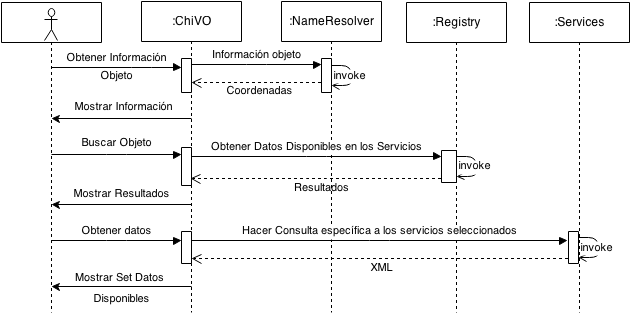
\includegraphics[width=0.45\textwidth]{images/secuencia.png}
    \caption{Diagrama de secuencia entre Usuario y ChiVO}
    \label{fig:secuencia}
\end{figure}

\subsection{Backend}
Dibujo de asdm -> ms -> fits \}metadata
Data Models

\begin{figure}[h]
    \centering
    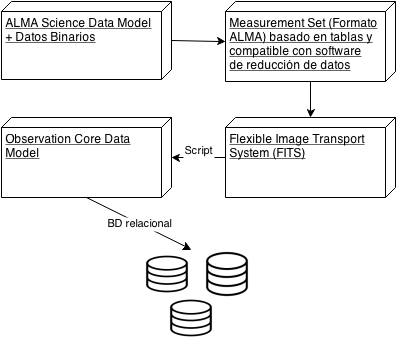
\includegraphics[width=0.45\textwidth]{images/metadata.png}
    \caption{Proceso transformación desde FrontEnd de ALMA hasta la base de datos de ChiVO}
    \label{fig:metadata}
\end{figure}



\subsection{Endpoint}
ChiVO Sesame, Registros externos.

\subsection{Frontend}
Tecnologías actuales
